\chapter{Root-finding decomposition}\label{sec:rootfinding}

\section{Origin: a suggestion in an audited manuscript}

The textbook decomposition oracle builds Semaev's polynomial system and
solves it with a Gr\"obner-basis engine. On 12 October a 13-page manuscript,
\emph{Point Decomposition by Root Finding}, was supplied for assessment. We
froze it (\art{research/ecbench_rootfinding_assessment_20261012/source-paper.pdf},
SHA-256 \texttt{743d3d3e\ldots7c01}) and audited it against its source
branch before measuring anything. Its central suggestion is simple: for two
summands, fixing one factor-base point turns $\Sem3$ into a quadratic in the
remaining variable whose roots are already known.

\begin{proposition}[roots of $\Sem3$]\label{prop:s3}
Let $E: y^2=x^3+ax+b$ over a field $K$ of characteristic $\ne2,3$, and let
$R,F\in E(K)$ be affine with $x_R\ne x_F$. Then
\[
  \Sem3(x_R,x_F,X)=(x_R-x_F)^2\,(X-x_+)(X-x_-),\qquad
  x_\pm=x(R\pm F),
\]
so $\Sem3(x_R,x_F,X)=0$ iff $X\in\{x(R+F),x(R-F)\}$.
\end{proposition}
\begin{proof}[Proof sketch]
With $\lambda_\pm=(\pm y_F-y_R)/(x_F-x_R)$ the chord slopes,
$x_\pm=\lambda_\pm^2-x_R-x_F$. Expanding $(X-x_+)(X-x_-)$ and eliminating
$y_R^2,y_F^2$ with the curve equation gives exactly Semaev's
$\Sem3/(x_R-x_F)^2$. The identity is machine-checked over an arbitrary
field in Lean 4 with Mathlib (\art{papers/rootfinding-decomposition/lean/S3Roots.lean},
theorems \texttt{SemaevS3.S3\_factor} and \texttt{SemaevS3.S3\_root\_iff};
no \texttt{sorry}; axioms \texttt{propext}, \texttt{Classical.choice},
\texttt{Quot.sound}).
\end{proof}

Hence the two-summand system has a parametrised variety: $R=\pm F_i\pm F_j$
iff $x(R\mp F_i)\in x(\Fb)$. No polynomial system is solved; the oracle is
one subtraction and one table probe per base point.

\paragraph{Prior art.} Neither the identity nor the oracle is new. The
identity is a direct consequence of how $\Sem3$ is defined: it is the
polynomial whose roots are the abscissae of $P_1\pm P_2$. The oracle
mechanism (sum $m-1$ factor-base points in the group and test whether the
result lies in the base) is the second algorithm of McGuire and
Mueller~\cite{mcguire2017}, who also evaluate $\Sem m$ by iterated
resultants instead of solving it, building on the instance-derived bases of
Amadori, Pintore and Sala~\cite{aps2018}. What this section adds is
engineering and measurement: a machine-checked proof, a fail-closed
verification protocol, binary pair-sum tables for up to four summands,
GPU, Kummer-tower and dense-index variants, and complete-cost measurements
in one harness against rho.

\paragraph{What the audit kept and corrected.} The identity is exact under
the stated generic affine condition, and a returned witness can be re-added
in the group for soundness. Completeness of the exhaustive enumeration
holds only with an explicit sign and factor-base convention (the binary
table stores full point keys over a base containing both signs; the
manuscript's schematic $x$-only table needed that convention stated). The
manuscript's NIST baseline was Buchberger, not F4
(\S\ref{sec:corrections}), and its statement that no implementation can
use fewer than linear field operations per ideal fails for repeated
queries against a reusable pair table. Larger-summand enumeration has a
growing exponent in $\abs\Fb$, and the manuscript did not benchmark it end
to end. All of this is recorded in
\art{research/ecbench_rootfinding_assessment_20261012/REPORT.md}.

\section{The algorithms}

\begin{algorithm}[t]
\caption[]{Prime two-summand oracle by direct subtraction}\label{alg:prime}
\begin{algorithmic}[1]
\Require target $R$, base $\Fb=\{F_1,\ldots,F_N\}$, hash set $H$ of
abscissae (or full points) of $\Fb$
\State $d_i\gets x_R-x_{F_i}$ for all $i$; invert all $d_i$ with one
  field inversion and $3(N-1)$ multiplications (Montgomery's trick)
\For{$i=1..N$}
  \For{$\varepsilon\in\{+1,-1\}$}
    \State $\lambda\gets(y_R+\varepsilon y_{F_i})\,d_i^{-1}$;\quad
           $x_3\gets\lambda^2-x_R-x_{F_i}$ \Comment{$x(R-\varepsilon F_i)$}
    \If{$x_3\in H$} recover the sign of $F_j$ from $y_3$; emit
      $R=\varepsilon F_i+\tau F_j$ \EndIf
  \EndFor
\EndFor
\end{algorithmic}
\end{algorithm}

\emph{Prime fields} (Algorithm~\ref{alg:prime},
\art{src/cryptanalysis/prime_fast.rs}): $\Theta(N)$ field operations and
$2N$ lookups per target. \emph{Binary fields}
(\art{src/cryptanalysis/koblitz_index_calculus.rs},
\texttt{DecompositionStrategy::PairTable}, made the default): a precomputed
table of pair sums $F_i+F_j$ turns an $m$-decomposition into $1$, $N$ or
$N^2$ lookups for $m=2,3,4$: the meet-in-the-middle half of a birthday
search, exact and complete like exhaustive search, at the price of
$\Theta(N^2)$ set-up and memory. Both are verified fail closed: every
decomposition is re-added in the group, $\Sem3$ is checked to vanish,
Gr\"obner-variety membership and agreement on refutation are checked
against F4, and planted positive controls must be found.

\section{Generalising the observation}

Over three days the identity was carried through every layer of the
pipeline. Table~\ref{tab:rf-steps} lists the steps; each is its own study
with a protocol registered before it ran.

\begin{table}[t]
\centering\small
\begin{tabularx}{\linewidth}{@{}>{\raggedright}p{3.1cm}X@{}}
\toprule
Step & What it adds; artefact \\
\midrule
Prime subtraction, binary pair table &
  Prop.~\ref{prop:s3}; batched inversion; $m\le4$ tables.
  \art{research/semaev_root_vs_groebner_20261012/} \\
NIST P-192\ldots P-521 &
  standard parameters, 6- and 64-point bases; dedicated P-256 field
  $11$--$12\times$ over generic big integers.
  \art{research/semaev_rootfind_nist_20261012/} \\
End to end vs msolve &
  complete DLPs with only the oracle swapped.
  \art{research/semaev_rootfind_e2e_20261012/} \\
PDP oracle family &
  \texttt{rf-mitm}, \texttt{mitm3}, \texttt{mitm4} (2-sum table);
  \texttt{rf-pairs}, \texttt{pairs3} (pairs then solve by the group law);
  \texttt{subtract2}; binary rungs $\ell=8..14$, prime Kummer towers
  $m=2,3,4$. \art{research/pdp_root_finder_20261012/} \\
CUDA kernel &
  one thread per (target, slice); per-thread Montgomery inversion; SoA
  base; shared-memory hash for $\abs\Fb\le2048$; 64-bit and P-256 fields.
  Checked in host emulation only until 12 November, then measured on an
  A100 (\S\ref{sec:rf-gpu}).
  \art{RESEARCH_GPU_ROOTFIND_DECOMPOSITION.md} \\
ecbench engines &
  \texttt{pdp3-koblitz:m=2|3,engine=rootfind}, \texttt{rootfind-subtract},
  later \texttt{rootfind-window} and \texttt{rootfind-negfold}.
  \art{research/ecbench_rootfind_engine_20261012/} and successors \\
Kummer-tower base &
  PKM's $\mu_{2^t}$ base with the root-finding oracles, 20--28-bit primes.
  \art{research/pkm_tower_ecbench_20261013/} \\
Dense root index, $n=83$ &
  packed five-byte $\Sem3$ root table, prefix widths K1271--K1798,
  8\,GiB of slots. \art{research/n83_dense_root_20261013/} \\
Prime tuning &
  pair-table size, arity, batched table inversions, synchronised lanes.
  \art{research/ecbench_rootfinding_\{tuning,arity,batchtable,lanes\}_2026101*/} \\
\bottomrule
\end{tabularx}
\caption[]{Root-finding generalisations, 12--14 October. Every row is
\cls{engineering}: no slope fell below its generic floor.}
\label{tab:rf-steps}
\end{table}

\section{Results}

\begin{figure}[t]
\centering
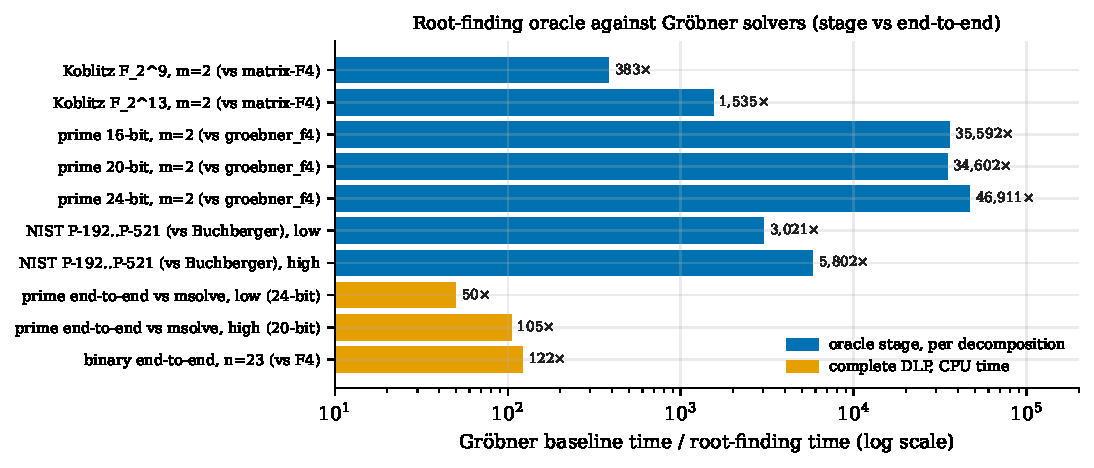
\includegraphics[width=\linewidth]{figures/fig-rootfind-oracle.pdf}
\caption[]{Root finding against Gr\"obner solvers on identical targets. Blue:
one decomposition (oracle stage only). Orange: complete discrete-log
computations with the oracle swapped and everything else fixed (prime: CPU
time against msolve, 20/24-bit totals composed from sampled per-query cost;
binary: one cold solve including table build). Sources:
\art{RESEARCH_SEMAEV_ROOTFIND_VS_GROEBNER.md},
\art{papers/rootfinding-decomposition/README.md}.}
\label{fig:rf-oracle}
\end{figure}

\paragraph{Oracle stage.} Per decomposition, root finding is
$383\times$ ($\FF_{2^9}$, $\abs\Fb=55$, 254 targets) and $1{,}535\times$
($\FF_{2^{13}}$, $\abs\Fb=4{,}005$, 256 targets) faster than matrix F4;
$3.5$--$4.7\cdot10^4\times$ faster than \texttt{groebner\_f4} on 16--24-bit
prime curves ($\abs\Fb=6$, 40 targets each); and $3{,}021$--$5{,}802\times$
faster than Buchberger on the decomposition ideal of the five NIST curves
(Figure~\ref{fig:rf-oracle}). Every binary verdict agreed with F4; every
prime solution was in F4's variety and every prime refutation was F4's unit
ideal. In the PDP study, \texttt{rf-mitm} refutes a binary target in
$3.1\,\mu$s at $\ell=8$ and $482\,\mu$s at $\ell=14$, against the PS-0
baseline's $9.3$\,ms and $55.5$\,s ($3{,}007$--$115{,}160\times$), costs
$5\abs\Fb-3$ multiplications and $2\abs\Fb$ lookups a target, and sits on
the pair-table floor at $1.000\pm0.027$ bits per rung; at prime $m=3$,
$N=18$ it uses 197 multiplications where F4 uses $8.99\cdot10^{13}$
multiply-adds; 707/707 brute-force agreements
(\art{research/pdp_root_finder_20261012/}).

Figure~\ref{fig:pf-rootfind} (left) and Table~\ref{tab:pf-rf-binary}
give the binary oracle rungs of the PDP study per target. From $\ell=8$
to $14$ the median wall of \texttt{rf-mitm} grows from $3.1$ to
$482.0\,\mu$s, and its lookups stay within $0.91$--$1.00$ of the pair-table
floor at every rung.

\begin{table}[t]
\centering\small
\setlength{\tabcolsep}{3.5pt}
\begin{tabular}{@{}rrrrrrrrrr@{}}
\toprule
& & \multicolumn{3}{c}{\texttt{rf-mitm} counts per target} & \multicolumn{4}{c}{median wall per target ($\mu$s)} & \\
\cmidrule(lr){3-5}\cmidrule(lr){6-9}
$n$ & $\ell$ & mults & lookups & /floor & \texttt{rf-mitm} & \texttt{rf-pairs} & group-scalar & baseline & baseline/\texttt{rf-mitm} \\
\midrule
23 & 8 & $592$ & $238$ & $0.93$ & $3.9$ & $202.2$ & $213.6$ & $8{,}698.1$ & $2{,}230.3$ \\
24 & 8 & $637$ & $256$ & $1.00$ & $3.1$ & $235.2$ & $276.5$ & $9{,}296.9$ & $3{,}007.2$ \\
27 & 9 & $1{,}262$ & $506$ & $0.99$ & $6.4$ & $879.0$ & $809.7$ & $37{,}705.5$ & $5{,}881.5$ \\
30 & 10 & $2{,}317$ & $928$ & $0.91$ & $10.7$ & $2{,}662.9$ & $2{,}693.2$ & $169{,}656.2$ & $15{,}801.8$ \\
33 & 11 & $5{,}032$ & $2{,}014$ & $0.98$ & $23.9$ & $12{,}462.9$ & $11{,}290.4$ & $707{,}969.2$ & $29{,}665.5$ \\
36 & 12 & $9{,}957$ & $3{,}984$ & $0.97$ & $57.6$ & $48{,}374.1$ & $48{,}094.4$ & $3{,}069{,}594.3$ & $53{,}254.7$ \\
39 & 13 & $20{,}257$ & $8{,}104$ & $0.99$ & $156.0$ & $206{,}909.0$ & $191{,}078.5$ & $13{,}115{,}950.2$ & $84{,}095.5$ \\
42 & 14 & $40{,}922$ & $16{,}370$ & $1.00$ & $482.0$ & $818{,}311.5$ & $757{,}478.1$ & $55{,}506{,}122.0$ & $115{,}160.1$ \\
\bottomrule
\end{tabular}
\caption[]{Root-finding decomposition oracles on binary curves, one
query per target. /floor: lookups over the pair-table floor. baseline:
the PS-0 enumeration; group-scalar: the same search by group arithmetic.
Median over 2--15 runs per cell (none contended). One oracle query, not a
complete discrete logarithm; wall clock on a shared host, descriptive.
Producer-reported; no validation file. Source:
\art{research/pdp_root_finder_20261012/ANALYSIS.json} (\texttt{binary});
extracted in \art{figures/data-pf-rootfind.json}.}
\label{tab:pf-rf-binary}
\end{table}

\paragraph{Complete solves.} End to end, the gain is two orders of
magnitude smaller and not one-sided: $50$--$105\times$ against msolve on
16--24-bit prime curves; $122\times$ on the one binary instance ($n=23$)
large enough to amortise the pair table; and F4 \emph{faster} at
$n=5,9,13$, where a solve needs too few decompositions to pay for the
table. Inside ecbench, with every group operation charged, the
root-finding IC beats inherited F4 in solve wall by about $350\times$ at
$n=13$ (admitted) and about $10^4\times$ at $n=23$ (descriptive), yet stays
$2.9$--$25{,}116\times$ the frozen strong rho in $S$ on Koblitz curves
$n=13$--$37$ (the jump at $n=31$ is mostly the curve's cofactor, 1{,}492) and
$29$--$141\times$ rho on prime curves, with the gap widening
(\art{research/pdp_root_finder_ecbench_20261013/}).

\begin{figure}[t]
\centering
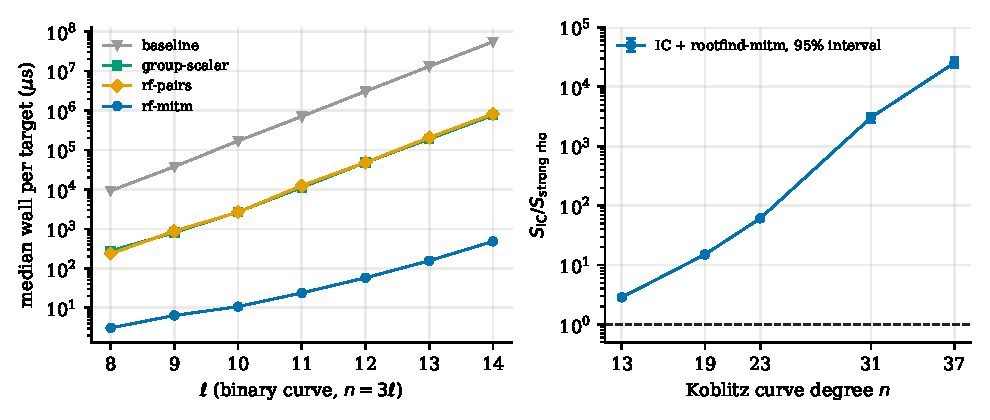
\includegraphics[width=\linewidth]{figures/fig-pf-rootfind.pdf}
\caption[]{Left: median wall per target of one decomposition query on
binary curves $n=3\ell$ (Table~\ref{tab:pf-rf-binary}). Right: counted
$S$ of the complete root-finding index calculus (\texttt{rootfind-mitm},
$m=3$) over the strong signed-Frobenius rho on Koblitz curves, with 95\%
cluster-bootstrap intervals (Table~\ref{tab:pf-rf-koblitz}); dashed:
parity. Producer-reported; no validation file. Data
\art{figures/data-pf-rootfind.json} from
\art{research/pdp_root_finder_20261012/ANALYSIS.json} and
\art{research/pdp_root_finder_ecbench_20261013/README.md}.}
\label{fig:pf-rootfind}
\end{figure}

\begin{table}[t]
\centering\small
\setlength{\tabcolsep}{4pt}
\begin{tabular}{@{}rrrrrrrl@{}}
\toprule
$n$ & strong rho & rho & IC+F4 & IC+\texttt{mitm} & IC+\texttt{rf-mitm} & IC+\texttt{rf-pairs} & \texttt{rf-mitm}/strong rho \\
\midrule
13 & $14.52$ & $1.88$ & $16.18$ & $32.80$ & $41.42$ & $300.8$ & $2.85$ $[2.64,3.04]$ \\
19 & $3.154$ & $0.752$ & $4.933$ & $39.89$ & $47.30$ & $1{,}886$ & $15.0$ $[14.3,15.7]$ \\
23 & $1.140$ & $0.457$ & $2.323$ & $66.31$ & $69.44$ & $7{,}648$ & $60.9$ $[56.1,66.0]$ \\
31 & $1.18$ & $0.37$ & --- & $3{,}599$ & $3{,}608$ & $1.8\cdot10^6$ & $3{,}053$ $[2{,}505,3{,}596]$ \\
37 & $0.240$ & $0.194$ & --- & $6{,}012$ & $6{,}016$ & --- & $25{,}116$ $[20{,}793,30{,}546]$ \\
\bottomrule
\end{tabular}
\caption[]{Root-finding index calculus on Koblitz curves in ecbench: mean
counted $S$ per arm, and \texttt{rootfind-mitm} over the strong
signed-Frobenius rho with a 95\% cluster-bootstrap interval. IC+F4 is a
lower bound (F4's word operations unpriced). rho: plain signed-Frobenius
rho. 40 runs per arm at $n=13,19$ and 24 at $n=23,31,37$. The jump at
$n=31$ is mostly the curve's cofactor, 1{,}492. Producer-reported; no
validation file. Source:
\art{research/pdp_root_finder_ecbench_20261013/README.md}; extracted in
\art{figures/data-pf-rootfind.json}.}
\label{tab:pf-rf-koblitz}
\end{table}

\paragraph{The Koblitz loops.} Figure~\ref{fig:k13} follows the best
complete-count root-finding arm at Koblitz $E_0$, $n=13$ through four
registered improvement loops (8 public targets $\times$ 3 rounds each, L0
operation counts). The first engine had $S=38.82$ ($m=3$) and $28.38$
($m=2$). A windowed third-summand scan cut $m=3$ by a paired $0.828$
$[0.783,0.863]$; a fold over negation (\texttt{rootfind-negfold}) took
$m=2$ to $23.22$ and then $22.97$. Two further cycles of denser and
sparser bases, windowed negfold and plain root finding were dead ends
(\art{research/ecbench_rootfind_vs_rho_20261014/}). With F4's word XORs
priced, the paired ratio negfold/F4 is $0.0545$ $[0.047,0.064]$, a
complete-against-complete comparison; against the frozen strong signed-Frobenius
rho ($S=14.82$) the best complete arm is still $1.55\times$. A compact-orbit
base with a counted Frobenius pair table reads $S=15.55$ against F4's
then-unpriced $16.75$ and about $1.06\times$ the strong rho. All three
figures are lower bounds (factor-base construction natives, F4's word XORs
and rho's table work unpriced), so neither order is ranked. Amortised over
64 targets the same arm reads $S\approx11.2$. That is a ratio of lower
bounds with no band, and the ledger counts it as a secondary, multi-target
diagnostic, not a result below rho
(\art{research/ecbench_rootfind_faster_20261014/README.md}).

\begin{figure}[t]
\centering
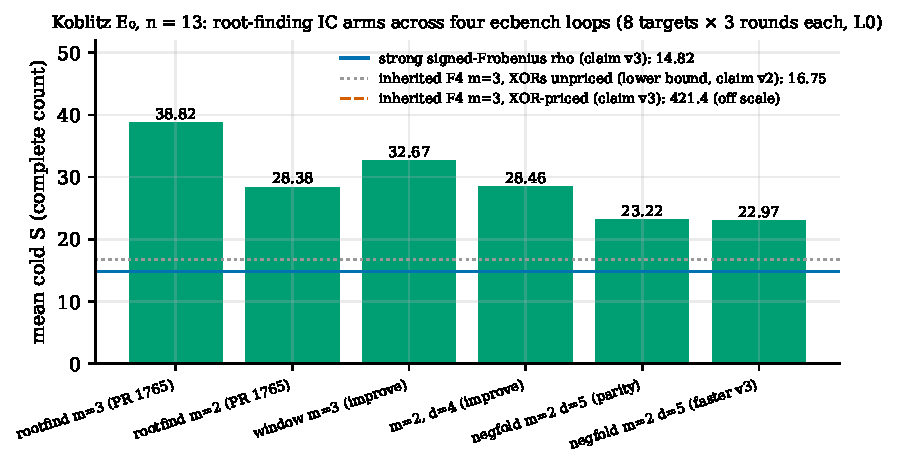
\includegraphics[width=\linewidth]{figures/fig-k13-progression.pdf}
\caption[]{Mean cold $S$ of root-finding IC arms at Koblitz $E_0$, $n=13$,
$d=5$ unless stated, across the engine, improve, parity and faster loops.
All bars are complete counts. Sources:
\art{research/ecbench_rootfind_engine_20261012/},
\art{research/ecbench_rootfind_improve_20261013/},
\art{research/ecbench_rootfind_parity_20261013/},
\art{research/ecbench_rootfind_faster_20261014/}. Each loop had its own
seeds and rho arm (rho $14.12$--$14.82$).}
\label{fig:k13}
\end{figure}

\paragraph{Prime tuning in ecbench.} On a 20-bit prime curve, the pair
table's counted $S$ is $0.018861$ $[0.018547,0.019242]$ of direct
subtraction (24 pairs; prime native work unpriced, so a bounded ratio), and
$0.057047$ $[0.041159,0.092069]$ on a 17-bit Koblitz curve, fully priced,
where the table set-up is about 68\% of the arm's cold cost. Doubling the
table from 32 to 64 abscissae gives $0.830$ $[0.697,0.962]$; three
summands instead of two costs $1.431\times$ $[1.225,1.716]$; batching the
table inversions leaves counted GAE unchanged ($1.000$; $4{,}096$ versus
$64$ inversions, set-up wall $243$ versus $128\,\mu$s, descriptive); and a
train-set lane selection did not resolve a hold-out winner ($0.979$
$[0.919,1.038]$; 1{,}088/1{,}088 executions with verified answers, sealed ecbench sessions)
(\art{benchmarks/README.md}, rows of 12--14 Oct).

\paragraph{Dense root index at $n=83$.} Widening the prefix base from
K1500 to K1798 cut mean probes per relation from $300{,}021.9$ to
$169{,}069.8$ (paired difference $130{,}952$, 95\% $[52{,}058,209{,}991]$)
and gave a one-point online ratio of $18.528$ over same-point rho (IC
$63.3$\,ms, rho $1{,}173.3$\,ms), with $339.0$\,s of reusable preparation
and an 8\,GiB table outside the window. The host was shared, so the result
is exploratory; two K1500 runs hit the 900\,s timeout and are retained.
The probe reduction stands; the online ratio does not: it was taken
against rho with an empty table, and rho with a precomputed table matched
to the index calculus's set-up is faster in every matched $n=83$ pair
(validation sweep, 20 October; \S\ref{sec:ladder2}).

\paragraph{Reading.} Root finding is the largest constant-factor change
of the programme at the oracle stage, and the one with a proof behind it.
It does not change the asymptotic count of index calculus: its cost is
$\Theta(\abs\Fb^{m-1})$, every measurement is at $m\le4$, and it leaves
relation yield, factor-base size and linear algebra untouched. Its effect
on the cold frontier is to move the decomposition stage from dominant to
minor, which exposes the stages that now are.

\section{Root finding on a GPU, 12--14 November}\label{sec:rf-gpu}

The CUDA kernel (one thread per target and slice) first ran on hardware on
12 November, on an A100 80\,GB PCIe, CUDA 12.8 (\S\ref{sec:in-gpuic}). The
audit's commits moved its time at $\abs\Fb=1{,}024$ from $23.53$ to
$19.91$\,ms and left $\abs\Fb=65{,}536$ unchanged ($0.995$--$1.000$); a fused
unwind and sweep was rejected, and the launch knobs stayed at their
defaults (\art{research/ic_gpu_measure_20261112/REPORT.md}). Every number
in this section is \texttt{[pcc:unverified]}.

\paragraph{Where the cycles go.} RunPod blocks the profiler counters, so
an instrumented build sampled \texttt{clock64()} at the phase boundaries of
one thread in 1{,}024 (\art{research/ic_gpu_replay_20261114/REPORT.md}).
Table probes took 62--85\% of the sampled cycles at $\abs\Fb=65{,}536$ and
41--60\% at $\abs\Fb=1{,}024$; the sweep's field arithmetic took 7.7--24.7\%. The
instrumented kernel runs $0.72$--$1.21\times$ the plain one's time, so the
split describes the instrumented kernel; that the lookups are bound by
memory latency is the source's interpretation.

\paragraph{Cheaper lookups.} Three changes keep the relation set and its
emission order: one 64-bit slot per hash entry (key tag and index, one load
per probe step), the two $\varepsilon$ lookups of a base entry issued
together, and an Eytzinger-ordered copy of the sorted keys. The host tests
found a bug in the first paired Eytzinger search (it read past the array
when the two descents left the tree at different levels); the new
primitive test fails with $3{,}610$ mismatches on the buggy version. Eight
builds, main twice as A/A, five rotated rounds at two workloads
(Table~\ref{tab:rf-gpu-lookup};
\art{research/ic_gpu_rootfind_lookup_20261114/REPORT.md}). An independent
validator recomputed every headline number from the raw tarball and
returned ``validated, scoped'': a kernel-time speed-up on one A100 at the
two workloads, with relation identity resting on device selftests, and four
wording corrections, applied in the source
(\art{research/ic_gpu_rootfind_lookup_20261114/VALIDATION_REVIEW.md}). The
three flags are on by default since 14 November.

\begin{table}[t]
\centering\small
\begin{tabular}{@{}lrr@{}}
\toprule
arm & $\abs\Fb=65{,}536$, $65{,}536$ targets & $\abs\Fb=1{,}024$, $262{,}144$ targets \\
\midrule
main (best configuration) & sorted/C16 $401.70$\,ms & hash/C16 $19.87$\,ms \\
Eytzinger & $1.050\times$ & $1.000\times$ \\
packed hash & $1.000\times$ & $1.112\times$ \\
paired & $0.999\times$ & $1.019\times$ \\
Eytzinger + paired & $1.116\times$ & $1.019\times$ \\
packed + paired & $1.000\times$ & $1.120\times$ \\
all three & $\mathbf{1.115\times}$ ($360.19$\,ms) & $\mathbf{1.121\times}$ ($17.73$\,ms) \\
\bottomrule
\end{tabular}
\caption[]{Root-finding lookup variants on one A100: main's best kernel
time over each arm's best, per workload, median of five rounds (61-bit
prime field). The A/A builds differ by at most $0.06\%$. Per
configuration, all three is faster than main at 12 of 12 configurations
($0.646$--$0.914$ of main's kernel time). A kernel-component result, no
counted-cost or rho claim. Validated (scoped) by an independent review;
\texttt{[pcc:unverified]}. Source:
\art{research/ic_gpu_rootfind_lookup_20261114/REPORT.md}.}
\label{tab:rf-gpu-lookup}
\end{table}

\paragraph{In a complete solve.} \texttt{rootfind-subtract-gpu} ($m=2$)
runs \texttt{rootfind-subtract}'s sweep on a persistent device session
and confirms each target's first hit through the CPU oracle; it is charged
exactly as the CPU oracle, and the extra device work is reported as
uncharged \texttt{gpu\_*} counters (\art{research/ic_gpu_rootfind_ic_20261114/REPORT.md}).
One frozen ecbench spec ran on 14 November on one A100 (AMD EPYC 9454
host): three prime-order curves of 28, 30 and 32 bits, two targets, two
rounds, prime-abscissa bases of $4{,}096$ and $16{,}384$, negation rho and an
A/A copy. All 72 records verified and replayed; all 24 CPU/GPU pairs have
equal $S$, logarithm, relations and relation-phase additions.

\begin{table}[t]
\centering\small
\begin{tabular}{@{}rrrrrrr@{}}
\toprule
$\log_2r$ & $\abs{\Fb_x}$ & mean $S$ & $S$/rho & CPU solve (s) & GPU solve (s) & relation phase, CPU/GPU \\
\midrule
27.5 & 4{,}096 & 6{,}259 & 6{,}403 & 1.88 & 0.489 & $25.8\times$ \\
27.5 & 16{,}384 & 3{,}639 & 3{,}723 & 2.72 & 1.07 & $21.4\times$ \\
30.0 & 4{,}096 & 18{,}007 & 13{,}154 & 12.4 & 0.507 & $84.4\times$ \\
30.0 & 16{,}384 & 14{,}371 & 10{,}498 & 12.1 & 1.39 & $77.8\times$ \\
31.3 & 4{,}096 & 26{,}010 & 22{,}986 & 28.0 & 0.643 & $113.2\times$ \\
31.3 & 16{,}384 & 23{,}265 & 20{,}560 & 28.6 & 1.51 & $121.2\times$ \\
\bottomrule
\end{tabular}
\caption[]{\texttt{rootfind-subtract} against \texttt{rootfind-subtract-gpu}
in complete prime-field index-calculus solves: $S$ is the same for both
arms; wall columns are medians of 4 paired runs (CPU arm one thread, GPU
arm one thread plus the device). $S$/rho is the distance remaining, and
it grows with $r$. The last column is the relation-phase wall ratio.
Validated (scoped) by an independent review, which re-verified all 88
certificates, replayed every record through a host-emulation worker and
refuted no number; L0, ecbench rates the wall comparison 0/100 with no
admitted pair; \texttt{[pcc:unverified]}. Sources:
\art{research/ic_gpu_rootfind_ic_20261114/REPORT.md},
\art{research/ic_gpu_rootfind_ic_20261114/VALIDATION_REVIEW.md}.}
\label{tab:rf-gpu-ic}
\end{table}

\noindent Table~\ref{tab:rf-gpu-ic} is a wall-time change on one host and
no counted-cost improvement. The GPU solve is now dominated by the worker
start and CUDA context ($0.25$--$0.35$\,s per solve, since ecbench runs each
record in a fresh process) and, at $\abs{\Fb_x}=16{,}384$, by the linear
algebra ($0.69$--$0.94$\,s on both arms). By a heuristic count, a two-summand
subtraction search does relation work that grows like $r$ against rho's
$\sqrt r$; the measured gap of $3{,}700$--$23{,}000\times$ grows with the
curve. Prefetching the next
Eytzinger level made the sorted path slower in every variant
($1.31$--$1.92\times$ at $\abs\Fb=65{,}536$, $1.21$--$1.81\times$ at $1{,}024$),
against A/A arms within $0.16\%$; the flag stays in the tree, off.

\section{Root finding on a GPU at $m=3$, 15 November}\label{sec:rf-gpu15}

Four rounds on single A100 80\,GB PCIe pods (CUDA 12.8) and three local
CPU studies took up the open items of \S\ref{sec:rf-gpu}: $m=3$ on the
device, the start-up paid by every solve, the linear algebra, and a
stronger multi-threaded CPU baseline. Every arm is charged as the CPU
oracle \texttt{rootfind-subtract}, so $S$ is unchanged by design, and it
was measured unchanged in every pair. Every record is L0
(\texttt{--cpus none --allow-busy}), and ecbench rates the wall
comparisons measurement quality 0/100 with no admitted pair; the wall
ratios below are descriptive, each measured on the named host, and
\texttt{[pcc:unverified]}. Independent validator reviews returned
``validated, scoped'' for rounds 2--5, for the linear-algebra study and for
the native-sweep study, each with corrections applied in its source; the
IFMA study has no validator. None of them adds a scoreboard or
leaderboard row. Every GPU record carries \texttt{work.complete: false}:
the device's sweep beyond the charged candidates, unused swept targets
and split batches are reported as uncharged \texttt{gpu\_*} counters.

\paragraph{Round 2: $m=3$ and a daemon.} \texttt{rootfind-subtract-gpu:m=3}
probes the abscissae of the negation-folded pair table that the CPU oracle
builds and charges, reports every hit, and confirms the reported
positions in order through the CPU probe, which reproduces
\texttt{rootfind-subtract:m=3}'s first hit and charge. With
\texttt{worker=daemon} one process holds the CUDA context ($0.376$\,s to a
ready context) and serves every run. All 232 records verified and
replayed, and 128 GPU/CPU pair checks found 0 mismatches. At $m=2$ and
$\abs{\Fb_x}=4{,}096$ the per-solve set-up medians fell from
$0.16$--$0.25$\,s to 2--4\,ms and the daemon's solve was
$20.8$--$127.8\times$ the one-thread CPU solve; part of its $2.0$--$3.5\times$
over a worker per run is a relation phase $0.054$--$0.058$\,s shorter. At
$m=3$ and $\log_2r=25.2$--$31.2$ the device was slower end to end
($0.41$--$0.86\times$ the CPU solve): sorting and shipping probe sets of
$1.02$--$4.19$ million abscissae added $0.12$--$0.15$\,s of set-up at
$\abs{\Fb_x}=1{,}024$ and $0.50$--$0.57$\,s at $2{,}048$. Its $S$ is
$43$--$672\times$ rho, against $5{,}800$--$22{,}000\times$ for $m=2$
(\art{research/ic_gpu_rootfind_m3_20261115/REPORT.md}).

\paragraph{Rounds 3 and 4: the tables on the device.} Round 3 (Intel Xeon
Gold 6240R host) filled the probe set's hash slots on the device, one
\texttt{atomicCAS} per key; added \texttt{backend=cuda|emulate}, where
\texttt{emulate} runs the kernel's per-thread code on host threads and is
the multi-threaded CPU arm; and generated \texttt{prime\_explicit}
prime-order curves of 34--40 bits, beyond \texttt{prime\_search}'s 32. At
37--39 bits the device took the $m=3$ relation phase from 8--32\,s to
$0.09$--$0.25$\,s, but at $\abs{\Fb_x}=4{,}096$ the CPU-built pair table
(about $16.8$ million sums) and the linear algebra (2.8--11\,s) left the
solve at $0.97$--$2.72\times$ the CPU's
(\art{research/ic_gpu_rootfind_big_20261115/REPORT.md}). Round 4 (AMD
EPYC 7543 host, cgroup quota $13.6$ CPUs) built the pair table on the
device: one thread per pair computes $x(P_a\pm P_b)$ in the CPU build's
order, a device hash keeps the least build index per abscissa
(\texttt{atomicMin}, the pair the CPU map's first insert keeps), and the
build is charged exactly as \texttt{PairTable::build\_negation\_folded}.
The device build's charge equals the CPU build's in all 36 records, and a
worker that reports the next build index fails the test ($7{,}299$
targets against 42). Table~\ref{tab:rf-gpu-pairs} gives the round
(\art{research/ic_gpu_rootfind_pairs_20261115/REPORT.md}).

\begin{table}[t]
\centering\small
\begin{tabular}{@{}rrrrrrrr@{}}
\toprule
& & & \multicolumn{2}{c}{CPU} & \multicolumn{2}{c}{GPU, pair table on} & set-up (s) \\
\cmidrule(lr){4-5}\cmidrule(lr){6-7}
$\log_2r$ & $\abs{\Fb_x}$ & $S$/rho & 1 thread & 14 threads & CPU & device & CPU $\to$ device table \\
\midrule
33.4 & 2{,}048 & 140 & 1.06 & 1.22 & 0.788 & 0.246 & $0.511\to0.034$ \\
35.2 & 2{,}048 & 166 & 1.86 & 1.29 & 1.02 & 0.260 & $0.496\to0.028$ \\
37.4 & 2{,}048 & 302 & 6.25 & 1.87 & 0.916 & 0.295 & $0.501\to0.018$ \\
39.3 & 2{,}048 & 569 & 21.1 & 4.00 & 0.949 & 0.368 & $0.505\to0.021$ \\
33.4 & 4{,}096 & 242 & 5.07 & 5.27 & 4.75 & 0.706 & $4.21\to0.124$ \\
35.2 & 4{,}096 & 142 & 5.41 & 6.35 & 5.87 & 1.36 & $2.94\to0.116$ \\
37.4 & 4{,}096 & 172 & 11.3 & 8.43 & 5.05 & 1.66 & $3.81\to0.109$ \\
39.3 & 4{,}096 & 298 & 24.8 & 7.38 & 5.78 & 1.49 & $2.92\to0.122$ \\
\bottomrule
\end{tabular}
\caption[]{Round 4: $m=3$ \texttt{rootfind-subtract} against its GPU arm
with the pair table built on the CPU or on the device; solve and oracle
set-up wall in seconds, medians of 4, one A100 pod with an AMD EPYC 7543
host. The device-table arm's solve is $4.0$--$57.3\times$ the one-thread
CPU solve; the CPU arm's A/A copy differs from it by up to 14\%. $S$/rho
($w=0$) is the distance remaining; the validator's band puts it at
$190$--$574\times$ at $w=0.1$ and $297$--$1{,}019\times$ at $w=1$, rho ahead
at every weight. Validated (scoped); \texttt{[pcc:unverified]}. Source:
\art{research/ic_gpu_rootfind_pairs_20261115/REPORT.md}.}
\label{tab:rf-gpu-pairs}
\end{table}

\paragraph{Linear algebra.} Round 4 left the linear algebra as most of the
device arm's solve at $\abs{\Fb_x}=4{,}096$. A local study (4-core Intel
Xeon VM) varied only the relation-matrix solver of
\texttt{rootfind-subtract:m=3}: \texttt{incremental-gauss}, the default of
every earlier round; \texttt{incremental-gauss-echelon}, sparse forward
elimination; and \texttt{structured-gauss}
(\art{research/ic_la_m3_20261115/REPORT.md}). All three pin the target
under the same completion rule, and all 24 comparisons have equal trials,
relations, logarithm, $S$ and relation-phase additions
(Table~\ref{tab:rf-la-m3}). The validator re-implemented both Gauss
solvers and found the saving in a second unit (\texttt{bitop/v1}). The
arms tie at $w=0$, so \texttt{ecbench band} rates every echelon/gauss pair
``unresolved inside the band''; at $w=0.1$ the echelon arm is
$1.03$--$1.82\times$ cheaper and at $w=1$ $1.15$--$3.81\times$, a count
difference that grows with the price of a native operation. The
validator's illustration at a calibrated $0.005$--$0.013$\,GAE per modular
multiplication puts it at $1.001$--$1.15\times$. \texttt{structured-gauss}
scans $2.7$--$7.8\times$ as many matrix entries as gauss, and its
linear-algebra wall is $0.50$--$0.88\times$ gauss's.

\begin{table}[t]
\centering\small
\begin{tabular}{@{}rrrrrrr@{}}
\toprule
& & \multicolumn{3}{c}{\texttt{row\_ops}} & LA wall (s) & cost/rho, $w=1$ \\
\cmidrule(lr){3-5}
$\log_2r$ & $\abs{\Fb_x}$ & gauss & echelon & structured & gauss $\to$ echelon & gauss $\to$ echelon \\
\midrule
33.4 & 2{,}048 & 46.6M & 6.9M ($0.15\times$) & 12.4M ($0.27\times$) & $0.194\to0.020$ & $168\to69$ \\
33.4 & 4{,}096 & 108.9M & 11.1M ($0.10\times$) & 27.8M ($0.26\times$) & $0.635\to0.037$ & $363\to118$ \\
35.2 & 2{,}048 & 43.6M & 5.8M ($0.13\times$) & 12.9M ($0.30\times$) & $0.214\to0.026$ & $2{,}196\to1{,}366$ \\
35.2 & 4{,}096 & 293.4M & 41.6M ($0.14\times$) & 72.7M ($0.25\times$) & $1.219\to0.115$ & $7{,}492\to1{,}966$ \\
37.4 & 2{,}048 & 42.3M & 5.9M ($0.14\times$) & 12.5M ($0.30\times$) & $0.246\to0.037$ & $836\to730$ \\
37.4 & 4{,}096 & 340.7M & 46.5M ($0.14\times$) & 99.4M ($0.29\times$) & $1.519\to0.135$ & $1{,}392\to537$ \\
\bottomrule
\end{tabular}
\caption[]{Linear algebra of $m=3$ \texttt{rootfind-subtract}: median
\texttt{row\_ops} per solver (deterministic counts) and indicative L0 wall,
one local 4-core VM, 2 targets per curve, one round. $S$/rho at $w=0$ is
$52$--$1{,}230$ and equal for the three solvers; the last column is the
\S\ref{sec:band} band at $w=1$ under \texttt{ecbench band}'s default
reading, as corrected by the validator (the first reading priced rho's
unpriced canonicalisations at 0). Validated (scoped);
\texttt{[pcc:unverified]}. Source:
\art{research/ic_la_m3_20261115/REPORT.md}.}
\label{tab:rf-la-m3}
\end{table}

\paragraph{Round 5: the echelon solver on the device.} The frozen
predictions held: equal identity in 84 checks, the GPU solve with echelon
at most $0.5\times$ its solve with gauss at $\abs{\Fb_x}=4{,}096$, and
\texttt{row\_ops} echelon/gauss $0.129$--$0.142$
(Table~\ref{tab:rf-gpu-la}; \art{research/ic_gpu_rootfind_la_20261115/REPORT.md}).
The linear algebra's share of the device solve at $4{,}096$ fell from
$0.87$--$0.89$ to $0.34$--$0.42$; set-up, linear algebra and relation phase
are now of one order. On the CPU the linear-algebra phase falls $9$--$11.5\times$
in wall, but the whole-solve difference ($0.79$--$0.98\times$) is not
resolved against relation-phase noise on identical counted work, and there
is no CPU A/A arm. Rho's median solve on one CPU thread is $0.040$\,s
($37.4$ bits) and $0.087$\,s ($39.3$ bits); the device echelon arm is
$2.6$--$7.1\times$ slower, and $5.4$--$13.2\times$ with the daemon's one-time
$0.242$\,s start. That sets an A100 against one CPU thread. The measured
binary is not bound to the measured commit by the records (the validator's
later build reproduces every worker-free record; the GPU arms' wall and
device path stay unbound).

\begin{table}[t]
\centering\small
\begin{tabular}{@{}rrrrrrrr@{}}
\toprule
& & & \multicolumn{2}{c}{CPU} & \multicolumn{2}{c}{GPU} & GPU echelon: \\
\cmidrule(lr){4-5}\cmidrule(lr){6-7}
$\log_2r$ & $\abs{\Fb_x}$ & $S$/rho & gauss & echelon & gauss & echelon & set-up / relations / LA \\
\midrule
37.4 & 2{,}048 & 340 & 5.66 & 5.39 & 0.287 & 0.118 & $0.038$ / $0.055$ / $0.023$ \\
37.4 & 4{,}096 & 194 & 8.09 & 6.40 & 1.551 & 0.280 & $0.122$ / $0.037$ / $0.117$ \\
39.3 & 2{,}048 & 737 & 20.2 & 19.7 & 0.387 & 0.223 & $0.032$ / $0.162$ / $0.024$ \\
39.3 & 4{,}096 & 383 & 20.0 & 17.8 & 1.541 & 0.305 & $0.121$ / $0.076$ / $0.104$ \\
\bottomrule
\end{tabular}
\caption[]{Round 5: $m=3$ solve wall in seconds (medians of 6) with
\texttt{incremental-gauss} and \texttt{incremental-gauss-echelon}, CPU on
one thread and GPU with the device pair table, one A100 pod (cgroup quota
$13.6$ CPUs). The GPU echelon arm's A/A copy is within $0.98$--$1.07\times$
per pair. $S$/rho is a ratio of means; the band for the GPU echelon arm at
$w=0$/$0.1$/$1$ is $340$/$342$/$350$, $194$/$206$/$261$, $737$/$738$/$742$
and $383$/$389$/$417$ (rows in order), rho ahead at every weight.
Validated (scoped); \texttt{[pcc:unverified]}. Source:
\art{research/ic_gpu_rootfind_la_20261115/REPORT.md}.}
\label{tab:rf-gpu-la}
\end{table}

\paragraph{CPU baselines.} Round 3's validator found the emulation arm
sweeping $1/7$--$1/9$ as many candidates per core as the one-thread Rust
arm (96 visible threads, unrecorded quota); round 4, with the pool sized
to the quota (14 threads), measured $7.5$--$10.5\times$ one thread at $m=2$.
\texttt{worker=native} sweeps each batch in process on a thread pool with
\texttt{rootfind-subtract}'s own scalar Montgomery arithmetic
(\art{research/ic_native_sweep_20261115/REPORT.md}). On a loaded 4-thread
Intel Xeon VM it reached $1.00$--$1.11\times$ the emulation arm's
relation-phase speed at $m=2$, where at least $1.5\times$ was predicted:
both arms reach $2.2$--$3.3\times$ one thread on four threads, and the
round-3 figure stays unexplained. With one thread the native sweep is
$0.56$--$0.93\times$ the plain arm, consistent with its sweeping
$1.02$--$2.16\times$ the candidates (every candidate of every target in a
lane round). \texttt{simd=ifma} runs eight targets per step, one per
AVX-512 lane, with $2^{52}$ Montgomery multiplication from
\texttt{vpmadd52luq}/\texttt{vpmadd52huq}; its lanes equal the scalar sweep
hit for hit, and 64 identity checks found 0 mismatches
(Table~\ref{tab:rf-ifma}; \art{research/ic_native_ifma_20261115/REPORT.md}).
At $m=2$ it is $1.60$--$1.67\times$ the scalar native sweep on one thread
and $1.50$--$1.62\times$ on four (the low end is $1.497$, at the predicted
$1.5\times$); at $m=3$, $1.25$--$1.44\times$, where each candidate probes a
64\,MiB set of pair-table abscissae at random.

\begin{table}[t]
\centering\small
\begin{tabular}{@{}rrrrrrrrr@{}}
\toprule
$m$ & $\log_2r$ & $\abs{\Fb_x}$ & one thread (s) & scalar $\times1$ & IFMA $\times1$ & scalar $\times4$ & IFMA $\times4$ & $S$/rho, $w=0$/$0.1$/$1$ \\
\midrule
2 & 27.5 & 4{,}096 & 2.01 & $0.79\times$ & $1.32\times$ & $3.09\times$ & $4.62\times$ & $6{,}690$/$6{,}706$/$6{,}781$ \\
2 & 30.0 & 4{,}096 & 11.4 & $0.94\times$ & $1.49\times$ & $3.47\times$ & $5.63\times$ & $16{,}809$/$16{,}830$/$16{,}922$ \\
3 & 33.4 & 2{,}048 & 0.436 & $0.52\times$ & $0.75\times$ & $2.09\times$ & $2.63\times$ & $213$/$296$/$668$ \\
3 & 35.2 & 2{,}048 & 1.74 & $0.95\times$ & $1.29\times$ & $3.49\times$ & $4.54\times$ & $150$/$171$/$264$ \\
\bottomrule
\end{tabular}
\caption[]{Native CPU sweeps of \texttt{rootfind-subtract-gpu} with
\texttt{worker=native}: the one-thread \texttt{rootfind-subtract} arm's
median relation-phase wall, and each arm's speed over it (scalar or IFMA,
1 or 4 threads; medians of 4), one local 4-thread Intel Xeon VM with
AVX-512 IFMA. The band columns hold for every IC arm; rho is ahead at every
weight. No validator; \texttt{[pcc:unverified]}. Source:
\art{research/ic_native_ifma_20261115/REPORT.md}.}
\label{tab:rf-ifma}
\end{table}

\paragraph{Reading.} Across rounds 3--5 the counted distance of $m=3$ to
the matched rho stays between $10^2$ and $10^3$ over the band ($107$--$1{,}019\times$
in rounds 3 and 4, $194$--$742\times$ in round 5). The device, the
daemon, the device tables, the echelon solver and the vector sweep change
wall time on the named hosts; only the echelon solver changes a count,
and that count is unpriced at $w=0$.
